\subsubsection{Summary}
Primarily, this microservice was fairly straightforward to develop. Most of the microservice was generated through \textit{Visual Studio}'s ability to scaffold controllers once models had been defined. A few behaviours needed more thought or needed discussion with the client, and are discussed below.

\subsubsection{Mapping Activities}

One of the first and main issues that were identified was that of how the application would handle normalising data from Fitbit and potentially other activity data providers. After some investigation, it was found that the Fitbit API didn't have a consistent format in how it returned what type of activity the user had performed; for example, Fitbit could return \textit{"Skiing 5\% slope"} and \textit{"Skiing 10\% slope"}. This lack of generalisation among activity types was identified as something that would cause the platform issues should other ingest services be developed in the future. 

Many solutions were discussed for this problem, such as having the application dynamically create activities as they were imported. Ultimately it was decided that the most robust solution which provided a consistent user experience would be to create a table which maps a variety of Fitbit activity identifiers onto a single \textit{Aber Fitness} activity (Fig. \ref{fig:health_mappings}). This idea was presented to the client and was implemented shortly after.

\begin{figure}[H]
    \centering
    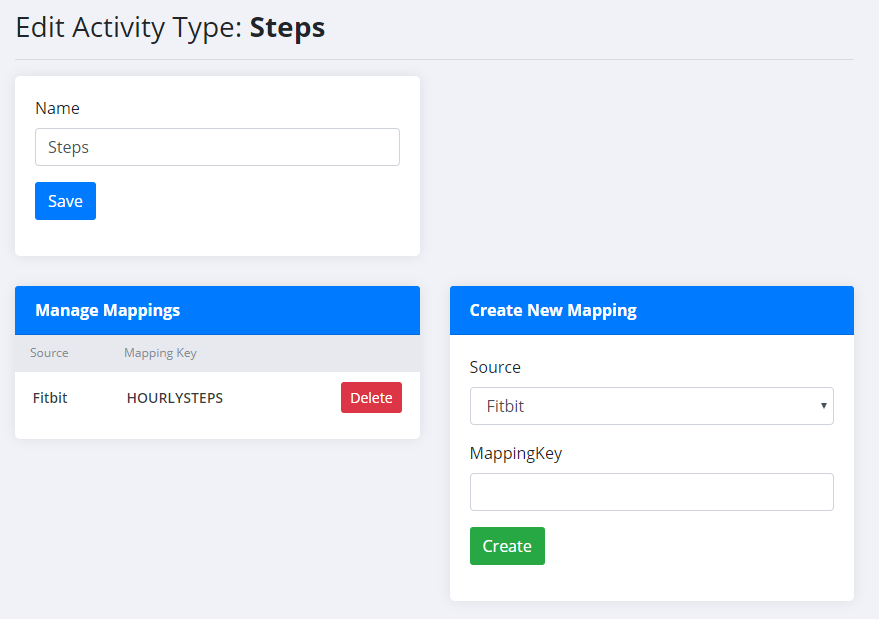
\includegraphics[width=0.7\textwidth]{Images/Chpt5_HealthData_Mapping.png}
    \caption{The administrative interface presented by \textit{Health Data Repository} which allows an administrator to create new mappings for activity types}
    \label{fig:health_mappings}
\end{figure}

The above interface was implemented into \textit{Aber Fitness} and provides an easily updated and flexible way for administrators to map custom external API activity identifiers onto internal activity resources. 

Ingest services are then offered an API endpoint by Health Data Repository which allows those services to retrieve the mapping table in order to determine the most appropriate Activity ID to map the data onto.

\subsubsection{Storing Step Data}
Initially, it was planned that the \textit{Fitbit Ingest Service} would be updating the \textit{Health Data Repository} with user's step counts on an hourly basis. In order to avoid an excessive quantity of activities being inserted into the database, it was decided that an activity would be created per day and updated hourly as steps came through from Fitbit. Therefore, it was required that an endpoint be available for step counts to be updated rather than inserting a new activity every hour. 

From experience with other MVC frameworks, it was assumed that .NET Core would have the ability to "Create Model, If Exists Update". This functionality is a standard part of SQL with the \lstinline{CREATE IF EXISTS UPDATE} syntax. It was surprising to find that .NET Core did not offer this functionality natively, and resulted in more code being written than was felt necessary had another framework been used. 

Ultimately this functionality was removed once it was discovered that we were unable to obtain step count data from Fitbit on an hourly basis, and therefore the additional API endpoints developed were no longer necessary. 